\documentclass[12pt,twoside]{article}
\usepackage{jmlda}	
% https://docs.google.com/document/d/1zkOK6iLzuwVahOh138aTh5FzoX_LHCWlMiGS1LnsZhA/edit
\title
%    [Автоматическая настройка параметров BigARTM ] % Краткое название; не нужно, если полное название влезает в~колонтитул
{Автоматическая настройка параметров BigARTM под широкий класс задач.}
\author
%    [Гришанов~А.\,В.] % список авторов для колонтитула; не нужен, если основной список влезает в колонтитул
{Гришанов~А.\,В., Булатов~B.\,Г., Воронцов~К.\,В.} % основной список авторов, выводимый в оглавление
[Гришанов~А.\,В.$^1$, Булатов~B.\,Г.$^1$, Воронцов~К.\,В.$^1$] % список авторов, выводимый в заголовок; не нужен, если он не отличается от основного
\thanks
%    {Работа выполнена при финансовой поддержке РФФИ, проект \No\,00-00-00000.
%   Научный руководитель:  Стрижов~В.\,В.
{Задачу поставил:  Булатов~B.\,Г.
	Консультант:  Воронцов~К.\,В.}
\email
{grishanov.av@phystech.ru, bt.uytya@gmail.com, vokov@forecsys.ru}
\organization
{$^1$ Московский физико-технический институт}%; $^2$Организация}
\abstract
{Открытая библиотека BigARTM позволяет строить тематические модели, используя широкий класс возможных регуляризаторов. При этом задача настройки коэффициентов оказывается весьма сложной. В данной статье мы ищем набор параметров, дающий <<достаточно хорошие>> результаты на широком классе задач, используя механизм относительных коэффициентов регуляризации и автоматический выбор N-грамм. Для эксперимента использовались наборы данных Victorian Era Authorship Attribution, 20 Newsgroups, МКБ-10. Модель с подобранными коэффициентами имеет качество не более чем на <X>\% хуже <<локально лучших моделей>>
	
	\bigskip
	\textbf{Ключевые слова}: \emph {тематическое моделирование, аддитивная регуляризация тематических моделей, PLSA, BigARTM}.}
\titleEng
{JMLDA paper example: file jmlda-example.tex}
\authorEng
{Author~F.\,S.$^1$, CoAuthor~F.\,S.$^2$, Name~F.\,S.$^2$}
\organizationEng
{$^1$Organization; $^2$Organization}
\abstractEng
{This document is an example of paper prepared with \LaTeXe\
	typesetting system and style file \texttt{jmlda.sty}.
	
	\bigskip
	\textbf{Keywords}: \emph{keyword, keyword, more keywords}.}
\begin{document}
	
	\maketitle
	
	\section{Введение}
	
	Тематические модели широко используются на практике для решения задач классификации и ранжирования документов, а также для разведочного поиска\cite{Ianina2016}. Одним из продвинутых инструментов в тематическом моделировании является библиотека BigARTM~\cite{vorontsov2015bigartm}. Она предоставляет широкий выбор для настройки модели, используя обширный класс регуляризаторов. Однако на практике популярнее остаются более простые методы, такие как LDA\cite{blei2003latent}. Во многом это связано со необходимостью аккуратного подбора параметров модели.
	
	Предлагается проверить гипотезу о существовании конфигураций, хорошо работающих на широком классе задач.
	
	Текущий подход к выбору параметров описан в работе \cite{Ianina2016}. Сначала подбирается один из регуляризаторов (например декоррелирования).  Его значение находится приблизительно, затем в зависимости от цели исследуется следующий параметр или продолжает улучшаться текущий. Существенно то, что имеются различные регуляризаторы  для различных итераций. Поэтому процесс перебора последовательный: добавляется один регуляризатор, оптимизируется, затем добавляется следующий. Из-за этого для оптимизации трудно использовать продвинутые методы, такие как байесовская оптимизация. Остаётся жадный или рандомизированный поиск.
	
	При этом возможны 2 типа коэффициентов: абсолютные и относительные. Первые не переносятся между разными коллекциями, для них заранее трудно предположить даже порядок оптимальных значений. Вторые более универсальны, но требуют дополнительных вычислений и менее стабильны.
	
	Цель данной работы --- исследовать процесс подбора параметров и найти критерии, по которым можно выбирать начальные конфигурации BigARTM для широкого класса задач. Предлагается использовать относительные коэффициенты регуляризации и автоматический подбор N-граммм.
	
	\section{Постановка задачи}
	
	Введем следующие обозначения:  $D$ --- коллекция текстовых документов, состоящая из документов d; W  словарь коллекции текстов, состоящий из термов $w$; $T$~--- множество тем, состоящее из тем  $t$.
	
	\subsection{Будем считать, что выполнены следующие гипотезы.}
	
	%\begin{enumerate}
	%\item
	Гипотеза о существовании тем. Каждое вхождение терма $w$ в документ $d$ связано
	с некоторой темой $t$ из заданного конечного множества $T$ . Коллекция документов
	представляет собой последовательность троек $\Omega_n = \left\{(w_i, d_i, t_i) : i=1,\dots \ n\right\}$. Термы $w_i$ и документы $d_i$ являются наблюдаемыми переменными, темы $t_i$ не известны
	и являются латентными (скрытыми) переменными.
	
	%\item 
	Гипотеза <<мешка слов>>. Порядок термов в документах не важен для выявления
	тематики, то есть тематику документа можно узнать даже после произвольной перестановки термов, хотя для человека такой текст потеряет смысл. Это предположение
	называют гипотезой <<мешка слов>> (bag of words). Порядок документов в коллекции
	также не имеет значения  это предположение называют гипотезой <<мешка документов>>.
	% Гипотеза <<мешка слов>> позволяет перейти к компактному представлению
	%документа как мультимножества  подмножества термов $d \subset W$ , в котором каждый терм $w \in d$ повторён $n_{dw}$ раз.
	
	%\item 
	Гипотеза условной независимости. Появление термов в документе $d$ по теме $t$ зависит от темы, но не зависит от документа $d$, и описывается общим для всех документов распределением $p(w|t)$:
	\begin{equation}
	p(w|d, t) = p(w|t).
	\end{equation}
	
	%\end{enumerate}
	
	\subsection{Вероятностная тематическая модель порождения текста.}
	Согласно формуле полной вероятности и гипотезе условной независимости, распределение термов
	в документе $p(w|d)$ описывается вероятностной смесью распределений термов в темах $\varphi_{wt} = p(w|t)$ с весами $\theta_{td} = p(t|d)$
	
	\begin{equation}\label{eq_0}
	p(w|d) = \sum\limits_{t \in T} p(w|t, d) p(t|d) = \sum\limits_{t \in T} p(w|t) p(t|d) = \sum\limits_{t \in T}\phi_{wt}\theta_{td}.
	\end{equation}
	
	Вероятностная модель (2) описывает процесс порождения коллекции по известным распределениям $p(w|t)$ и $p(t|d)$. Этот процесс показан на рис. 1.
	
	\begin{figure}[h]
		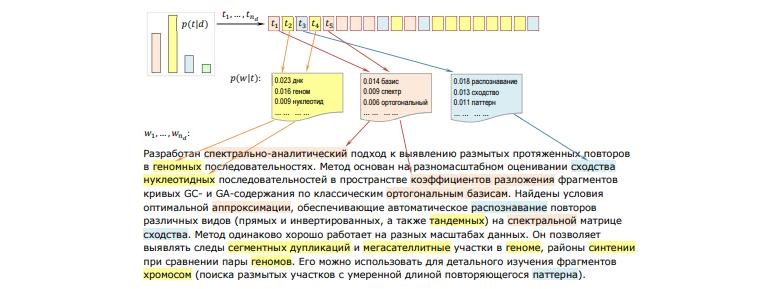
\includegraphics[scale=0.6]{generation}
		\caption{Процесс порождения текстовой коллекции вероятностной тематической моделью (2): в каждой позиции $i$ документа $d_i$ сначала порождается тема $t_i \sim p(t|d_i)$, затем терм $w_i \sim p(w|t_i)$}
		\label{fg:generation}
	\end{figure}
	
	\subsection{Задача тематического моделирования --- это обратная задача.} По заданной коллекции $D$ требуется найти параметры $\varphi_{wt}$ и $\theta_{td}$ , при которых тематическая модель (2)
	хорошо приближает частотные оценки условных вероятностей \newline $\hat{p}(w|d)=\frac{n_{dw}}{n_d}$. Распределение вида $p(t|x)$ будем называть тематикой объекта x. Можно говорить о тематике документа $p(t|d)$, терма $p(t|w)$, терма в документе $p(t|d, w)$.
	Целью тематического моделирования является определение тематики документов
	и связанных с ними объектов. Также требуется находить распределения $\varphi_{wt}= p(w|t)$,
	описывающие семантику каждой темы t словами естественного языка.
	
	Равенство (2) можно переписать в матричном виде. В левой части равенства находится известная матрица частот термов в документах $F=(\hat{p}(w|d))_{W \times D}$. Ставится задача разложения матрицы $F$ в произведение двух матриц $\Phi$ и $\Theta$ меньшего размера, таких, что
	\begin{gather*}
	\Phi = (\phi_{wt})_{W \times T}, \; \phi_{wt} = p(w|t)      \text{ --- матрица <<термины-темы>>}\\
	\Theta = (\theta_{td})_{T \times D}, \; \theta_{td} = p(t|d)  \text{ --- матрица <<темы-документы>>}
	\end{gather*}
	
	\begin{figure}[h]
		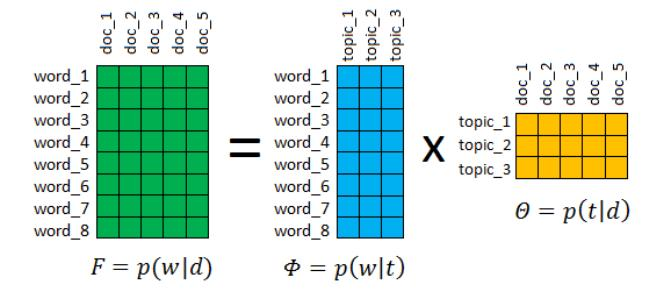
\includegraphics[scale=0.7]{decomposition}
		\caption{Иллюстрация матричного разложения.}
		\label{fg:Example}
	\end{figure}
	
	%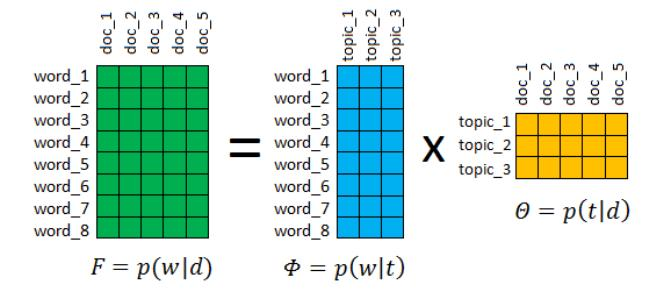
\includegraphics[scale=0.6]{decomposition.jpg}
	
	Поставленная задача ($F \approx \Phi \Theta$) эквивалентна поиску матриц $\Phi$ и $\Theta$, максимизирующих следующий функционал правдоподобия:
	
	\begin{equation}\label{eq_1}
	L(\Phi, \Theta) = \sum_{d \in D} \sum_{w \in d} n_{dw} \sum_{t \in T} \phi_{wt} \theta_{td} \rightarrow \max_{\Phi, \Theta}
	\end{equation}
	
	Заметим, что если $\Phi \Theta$ --- решение, то $(\Phi S ) (S^{-1}\Theta)$ --- также является решением для всех невырожденных матриц $S$. Неоднозначность матричного разложения  $F \approx \Theta \Phi$ порождает неоднозначность в
	выборе матриц из правой части равенства. Для решения данной проблемы, наложим
	на тематическую модель дополнительные требования. Модифицируем максимизирующий функционал:
	
	\begin{equation}
	L(\Phi, \Theta) + R(\Phi, \Theta) \rightarrow \max_{\Phi, \Theta}
	\end{equation}	
	\begin{equation}	
	R(\Phi, \Theta) = \sum_{j=1}^{n} \tau_j R_j(\Phi, \Theta)
	\end{equation}
	где $R_j(\Phi, \Theta)$ --- дополнительные требования к модели (регуляризаторы),  $\tau_j$ --- неотрицательные коэффициенты регуляризации. Полученный подход к построению тематических моделей имеет название АРТМ (аддитивная регуляризация тематических моделей).
	
	\subsection{Критерии качества}
	
	Для оценки качества использовались как внутренние, так и внешние критерии качества.
	
	Внутренние оценивают качество построенной модели по матрицам $\Phi$ и $\Theta$, которые в итоге дала модель.
	В качестве таких использовались перплексия и разреженность полученных матриц $\Phi$ и $\Theta$. Они вычислялись на всех датасетах.
	
	Внешние критерии измеряют качество полученных предсказаний. Из внешних критериев использовались точность и f-мера. Они использовались на размеченных наборах данных
	
	\subsection{Итоговая постановка}
	
	Рассмотрим набор датасетов $\left\{\mathfrak{D}_{ex}, \mathfrak{D}_{in}\right\}$, где  $\mathfrak{D}_{ex} = \left\{\mathfrak{D}_j\right\}_{j=1}^{N_{ex}}$ имеют внешний критерий качества $S(\tau_j, \mathfrak{D}_j)$, а $\mathfrak{D}_{in} = \left\{\mathfrak{D}_j\right\}_{j=1}^{N_{in}}$~ --- только внутренние. Для каждого из первых найдём лучшие параметры.
	
	\begin{equation}
	\tau_{j_{best}} = \argmin_{\tau} S(\tau, \mathfrak{D}_j) ,\ j = 1,\dots , N_{ex}
	\end{equation}
	
	Необходимо проверить гипотезу о том, что существуют коэффициенты регуляризации $\tau_{general}$, которые можно считать <<универсальными>>, т.е. такие что выполнено:
	
	\begin{equation}
	\max_{j=1,\dots,N_{ex}+N_{in}} \frac{S(\tau_{j_{best}}, \mathfrak{D}_j)- S(\tau_{general}, \mathfrak{D}_j)}{S(\tau_{j_{best}}, \mathfrak{D}_j)} \leq 5\%
	\end{equation}
	
	Для поиска $\tau_{general}$ будем использовать $\mathfrak{D}_{ex}$, минимизируя следующий функционал:
	
	\begin{equation}
	\sum_{j=1}^{N_{ex}} \left(S(\tau_{j_{best}}, \mathfrak{D}_j)- S(\tau_{general}, \mathfrak{D}_j)\right)^2 \to \min
	\end{equation}
	
	Гипотезу (7) будем проверять на $\left\{\mathfrak{D}_{ex}, \mathfrak{D}_{in}\right\}$. Для этого дополнительно введём следующие определения для наборов данных с внутренними критериями качества:
	
	\begin{Def}
		Модель $X$ {\bf не хуже} чем модель $Y$, если по всем критериям $X$ хуже не более чем на $5\%$.
	\end{Def}
	
	\begin{Def}
		Модель $X$ {\bf лучше} модели $Y$ по $k$ критериям, если по этим $k$ критериям $X$ лучше $Y$ хотя бы на $5\%$.
	\end{Def}
	
	Цель работы --- построить модель, которая {\bf не хуже} чем PLSA\cite{Hofmann:1999:PLS:2073796.2073829} и {\bf лучше} PLSA по нескольким критериям.
	
	\newpage
	
	\section{Относительные коэффициенты регуляризации}
	
	Формула M-шага, сглаживающего ($\tau > 0$) или разреживающего ($\tau < 0$) распределение
	$\varphi_{wt}$:
	
	\begin{equation}
	\varphi_{wt} = \underset{w \in W}{\text{norm}} \left(n_{wt} + \tau \right)
	\end{equation}
	
	
	Интуитивный смысл этого преобразования прост: мы либо <<притягиваем>> Фи к равномерному распределению $\beta = \frac{1}{|W|}$, либо ”отталкиваем” её от него же (возможно, даже
	зануляя при этом какие-то компоненты).
	Оказывается, можно провести репараметризацию, которая строго это продемонстрирует.
	
	Пусть $\beta = \frac{1}{|W|}$ — равномерное распределение, а текущие значения $n_{wt}$ и $\tau \in \mathbb {R}$ таковы, что на этой итерации M-шага зануления компонент не происходит (то есть либо $\tau > 0$,
	либо $\tau < 0$, но $n_{wt} + \tau > 0$).
	Тогда операцию положительной обрезки можно проигнорировать:
	\begin{equation}
	\varphi_{wt} = \underset{w \in W}{\text{norm}} \left(n_{wt} + \tau \right) = \frac{n_{wt} + \tau}{\sum\limits_{w \in W} n_{wt} + \tau} = \frac{n_{wt} + \tau}{n_{t} + \tau |W|}
	\end{equation}
	
	Попробуем представить это выражение, как выпуклую комбинацию распределений $\frac{n_{wt}}
	{n_t}$ (оценки максимума правдоподобия) и $\frac{1}{|W|}$ (равномерного распределения).
	
	\begin{equation}
	\frac{n_{wt} + \tau}{n_{t} + \tau |W|} = (1 - \lambda)\frac{n_{wt}}{n_t} + \lambda \frac{1}{|W|} 
	\Rightarrow
	\tau = \frac{n_t\lambda}{(1 - \lambda)|W|}
	\end{equation}
	
	Значит, сглаживание Фи можно трактовать, как нахождение компромисса между $\varphi_{wt}$~=~$\frac{n_{wt}}
	{n_t}$ и $\varphi_{wt} = \frac{1}{|W|}$.
	
	Допустим, мы хотим провести регуляризацию так, чтобы $\varphi_{wt}$ на 50\% состояла из оценки максимума правдоподобия, и на 50\% из априорного
	распределения $\frac{1}{|W|}$. Для этого достаточно вычислить $\tau$ по формуле и подставить в модель.
	
	%\subsection{Используемые регуляризаторы} \label{subsec:coefs}
	%
	%Будем использовать следующие 5 регуляризаторов:
	%
	%\begin{enumerate}
	%	
	%	\item 
	%	Сглаживание распределений терминов в темах. 
	%	
	%	Используется для выделения фоновых тем, собирающих общую лексику языка или общую лексику данной коллекции.
	%	
	%	\item 
	%	Сглаживание распределений тем в документах. 
	%	
	%	Используется для выделения фоновых слов в каждом документах.
	%	
	%	\item 
	%	Разреживание распределений терминов в темах. 
	%	
	%	Используется для выделения лексических ядер предметных тем как относительно небольшой доли слов словаря.
	%	
	%	\item 
	%	Разреживание распределений тем в документах. 
	%	
	%	Используется для выделения относительно небольшой доли предметных тем в каждом документах.
	%	
	%	\item 
	%	Декоррелирование распределений терминов в темах. 
	%	
	%	Используется для повышения различности лексических ядер предметных тем.
	%	
	%\end{enumerate}
	
	%\begin{State}
	%    Мотивации и~интерпретации наиболее важны для понимания сути работы.
	%\end{State}
	
	%\begin{Theorem}
	%    Не~менее $90\%$ коллег, заинтересовавшихся Вашей статьёй,
	%    прочитают в~ней не~более~$10\%$ текста.
	%\end{Theorem}
	%
	%\begin{Proof}
	%    Причём это будут именно те~разделы, которые не содержат формул.
	%\end{Proof}
	%
	%\begin{Remark}
	%    Выше показано применение окружений
	%    Def, Theorem, State, Remark, Proof.
	%\end{Remark}
	
	
	%\section{Заключение}
	
	%Желательно, чтобы этот раздел был, причём он не~должен дословно повторять аннотацию.
	%Обычно здесь отмечают,
	%каких результатов удалось добиться,
	%какие проблемы остались открытыми.
	
	
	\bibliographystyle{plain}
	\bibliography{Grishanov2019Project4}
	%\begin{thebibliography}{1}
	%
	%\bibitem{author09anyscience}
	%    \BibAuthor{Author\;N.}
	%    \BibTitle{Paper title}~//
	%    \BibJournal{10-th Int'l. Conf. on Anyscience}, 2009.  Vol.\,11, No.\,1.  Pp.\,111--122.
	%\bibitem{myHandbook}
	%    \BibAuthor{Автор\;И.\,О.}
	%    Название книги.
	%    Город: Издательство, 2009. 314~с.
	%\bibitem{author-and-co2007}
	%    \BibAuthor{Автор\;И.\,О., Соавтор\;И.\,О.}
	%    \BibTitle{Название статьи}~//
	%    \BibJournal{Название журнала}. 2007. Т.\,38, \No\,5. С.\,54--62.
	%\bibitem{bibUsefulUrl}
	%    \BibUrl{www.site.ru}~---
	%    Название сайта.  2007.
	%\end{thebibliography}
	
	% Решение Программного Комитета:
	%\ACCEPTNOTE
	%\AMENDNOTE
	%\REJECTNOTE
\end{document}
